\documentclass[main]{subfiles}


\begin{document}
\newpage
\section{Learning In Recurrent Neuronal Networks (RNNs)}
\subsection{Motivation: Why is it so important to understand RNN learning?}
\begin{enumerate}
    \item The mammalian cortex is highly recurrent - it will help us to better understand the brain.
    \item The core reason that recurrent nets are more exciting is that they allow us to operate over sequences of vectors: Sequences in the input, the output, or in the most general case both. Thus better understanding RNNs might help us to develop new, powerful RNN algorithms that are able to learn long and complex sequences.
    \item In programming terms be interpreted as running a fixed program with certain inputs and some internal variables. Viewed this way, RNNs essentially describe programs. In fact, it is known that RNNs are Turing-Complete in the sense that they can be used to simulate arbitrary programs (with proper weights).
    \item RNNs perform exceptionally well in language-modeling, the task of predicting the probability of the next word in a sequence.
\end{enumerate}


\subsection{RNNs in machine learning}
\subsubsection{What is a Recurrent Neural Network? (RECAP)}
\begin{figure}[H]
    \centering
    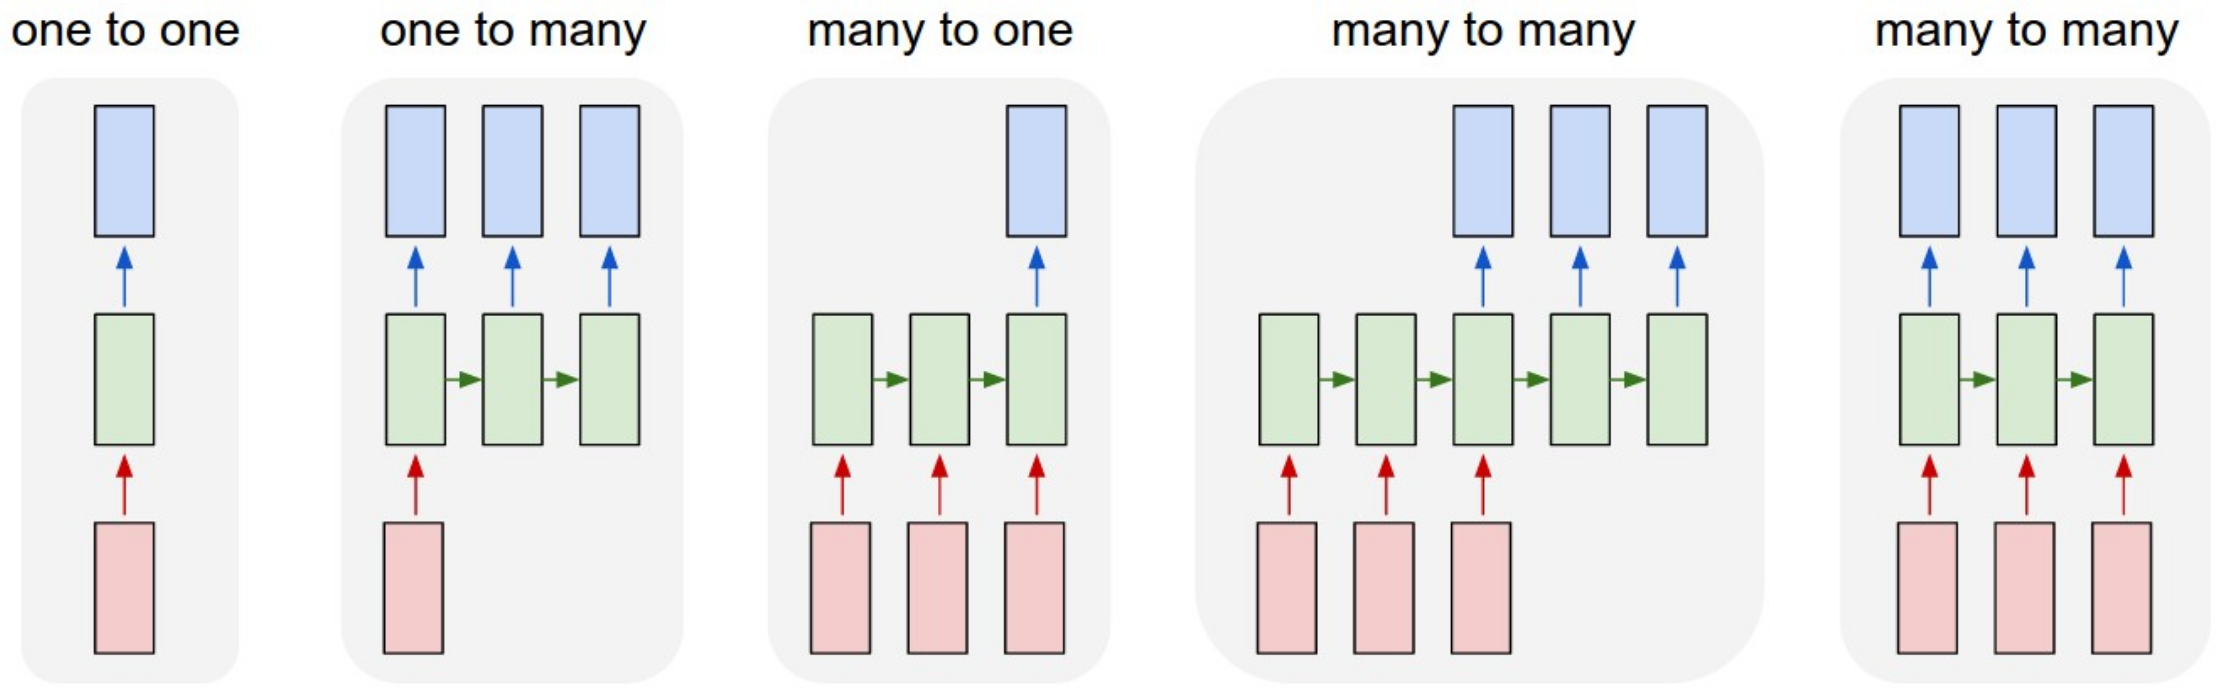
\includegraphics[width=0.99\linewidth]{13_LearningInRecurrentNeuronalNetworks/figures/onetomany.png}
    \caption{Each rectangle is a vector and arrows represent functions (e.g. matrix multiply). Input vectors are in red, output vectors are in blue and green vectors hold the RNN's state (more on this soon). From left to right: \textbf{(1)} Vanilla mode of processing without RNN, from fixed-sized input to fixed-sized output (e.g. image classification). \textbf{(2)} Sequence output (e.g. image captioning takes an image and outputs a sentence of words). \textbf{(3)} Sequence input (e.g. sentiment analysis where a given sentence is classified as expressing positive or negative sentiment). \textbf{(4)} Sequence input and sequence output (e.g. Machine Translation: an RNN reads a sentence in English and then outputs a sentence in French). \textbf{(5)} Synced sequence input and output (e.g. video classification where we wish to label each frame of the video). Notice that in every case are no pre-specified constraints on the lengths sequences because the recurrent transformation (green) is fixed and can be applied as many times as we like.}
    \label{fig:onetomany}
\end{figure}


Recurrent Neural Networks (RNNs) add an interesting twist to basic neural networks. A vanilla neural network takes in a fixed size vector as input which limits its usage in situations that involve a ‘series’ type input with no predetermined size. Recurrent nets allow us to operate over sequences of vectors: Sequences in the input, the output, or in the most general case both (A sequence means, that the elements can have dependency on each other and that the order matters!). A few examples that may make this more concrete\footnote{Cool blog by Karpathy (Teslas AI director): \url{http://karpathy.github.io/2015/05/21/rnn-effectiveness/}}, are shown in \cref{fig:onetomany}. The size of the input or output sequence is flexible, i.e. does not change the architecture of the model. Each network state gets an indices for the sequence. Since the sequence is often related with time progression, the index is choosen to be $t$. The main difference in architecture compared to conventional ANNs is, that recurrent loops are allowed, i.e. inputs from previous layer states of the network. Looking at a one-to-one neural network with one hidden layer, we can write the output state $y(t)$ and the hidden layer state $h(t)$ as follows:

\begin{align*}
    y(t) &= g_y(W_y h(t) + b_y) \tag{1}\\
    h(t) &= g_h(W_x x(t) + W_h h(t-1) + b_h) \tag{2}\\
    &= g_h((W_{hh}W_{xh}) \myvec{h_{t-1}\\ x_t})\\ 
    &= g_h(W \myvec{h_{t-1}\\ x_t}),
\end{align*}
where we include the bias in the W matrix. If we want to display the network over all sequences graphically, i.e. the computational graph, we can unroll it as displayed in \cref{fig:unroll}. 

\begin{figure}[H]
    \centering
    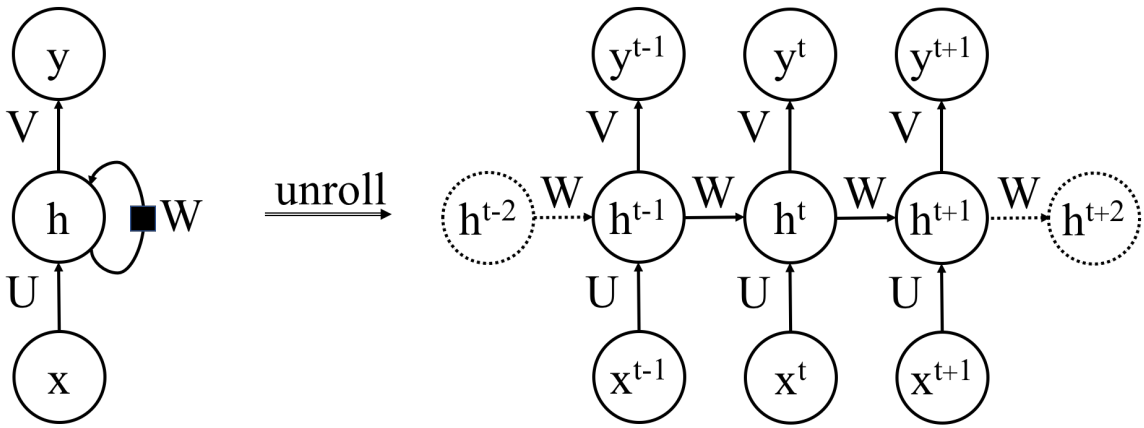
\includegraphics[width=0.99\linewidth]{13_LearningInRecurrentNeuronalNetworks/figures/unrolling.png}
    \caption{Computational graph of a many-to-many network: Unrolling the network over all sequences.}
    \label{fig:unroll}
\end{figure}

This gives us another perspective: For any fixed sequence length $s$, the unrolled recurrent network corresponds to a feedforward network with $s$ hidden layers. The two main differences to a feedforward network is, that the inputs are processed and outputs produced in sequence, and that the same parameters are used for all layers / all time steps, i.e. the same functions $U$, $V$, $W$ applied over all time steps\footnote{Here another helpful entry: \url{https://towardsdatascience.com/recurrent-neural-networks-d4642c9bc7ce}}(Not to be confused with all epochs!!!).

\subsubsection{Back-Propagation Through Time (BPTT)}
The unfolding shown in \cref{fig:unroll} is the first step of a particular network training algorithm, which is called Back-Propagation Through Time (BPTT). The second step is applying our known backpropagation algortihm to the unrolled network to calculate all weight updates. 
%
\begin{figure}[H]
    \centering
    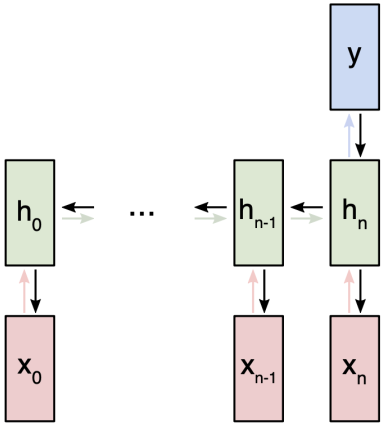
\includegraphics[width=0.5\linewidth]{13_LearningInRecurrentNeuronalNetworks/figures/bptt.png}
    \caption{Illustrating the backpropagation-through-time algorithm on a many-to-one RNN.}
    \label{fig:unroll}
\end{figure}
%
There are several drawbacks to BPTT:
\paragraph{Costly parameter update:} Especially for long sequences, the parameter update for a shallow layer is the same as updating a parameter in an extremely deep feedforward network. One way to fix this is using a truncated BPTT algortithm.  It processes the sequence one timestep at a time, and every $k1$ timesteps, it runs BPTT for $k2$ timesteps, so a parameter update can be cheap if $k2$ is small. Consequently, its hidden states have been exposed to many timesteps and so may contain useful information about the far past, which would be opportunistically exploited\footnote{Sutskever, "Training Recurrent Neural Networks", 2013}.

\paragraph{Exploding gradients:} The gradients coming from the deeper layers have to go through continuous matrix multiplications because of the the chain rule, and as they approach the earlier layers. If they have large values ($>1$) they get larger and eventually blow up and crash the model (NaN-values!). This can be solved by gradient clipping; which places a predefined threshold on the gradients to prevent it from getting too large. Note that this only changes the length, and not the direction, of the gradients.

\paragraph{Vanishing gradients:} A similar problem arises if the gradients have small values ($<1$). They will shrink exponentially until they vanish and make it impossible for the model to learn. This issue cannot be solved as simple; hence it requires to use shorter sequences or to make fundamental change in the RNN architecture. 


\subsubsection{Long-Short-Term-Memory (LSTM) Networks}
Long Short-Term Memory (LSTM) is a feature of a RNN that tackles the problems arising from long sequences / deep networks by a clever memory management\footnote{Hochreiter\&Schmidhuber, "Long Short-Term Memory", 1997} \footnote{Great blog post explaining LSTM: \url{http://colah.github.io/posts/2015-08-Understanding-LSTMs/}}. A common LSTM unit is composed of a cell, an input gate \textbf{i}, an output gate \textbf{o}, a forget gate \textbf{f} and a gate gate \textbf{g}. The cell remembers values over arbitrary time intervals and the three gates regulate the flow of information into and out of the cell. A comparison between a normal RNN cell and a LSTM cell is given in the figure below.  
\begin{figure}[H]
    \centering
    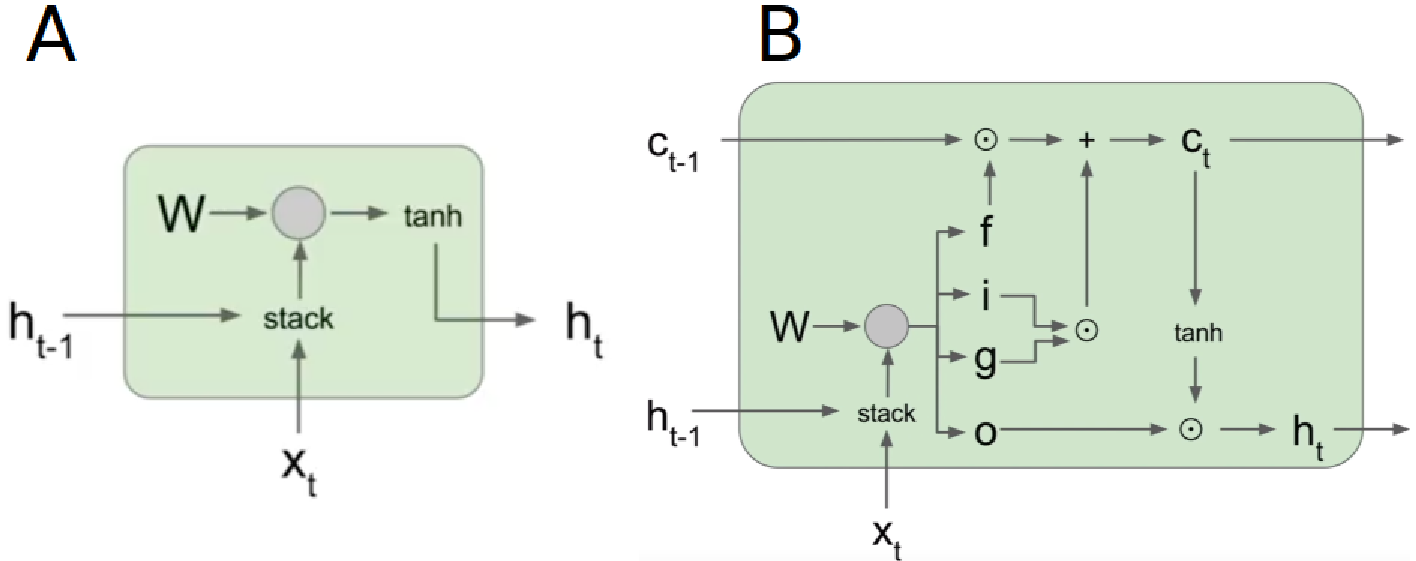
\includegraphics[width=0.99\linewidth]{13_LearningInRecurrentNeuronalNetworks/figures/lstm.png}
    \caption{A comparison between a normal RNN cell \textbf{A} and a LSTM cell \textbf{B}.}
    \label{fig:unroll}
\end{figure}
The gate vector can be written as 
\begin{equation*}
    \myvec{i\\ f\\ o\\ g} = \myvec{\sigma\\ \sigma\\ \sigma\\ \tanh} W \myvec{h_{t-1}\\ x_t}, \tag{3}
\end{equation*}
where $W = \myvec{W_i& W_f& W_o& W_g}.$ The cell state is defined as the following:
\begin{align*}
    c_t = & f \odot c_{t-1} + i \odot g \\ \tag{4}
    = &\sigma ( W_{hf} h_{t-1} + W_{xf} x_t ) \odot c_{t-1}\\ 
    + &\sigma ( W_{hi} h_{t-1} + W_{xi} x_t ) \odot \tanh (W_{hg} h_{t-1} + W_{xg} x_t)
\end{align*}
The hidden state is then given by 
\begin{align*}
    h_t &= o \odot \tanh(c_t)\\ \tag{5}
    &= \sigma (W_{hho} h_{t-1} + W_{xho} x_t ) \odot \tanh(c_t)
\end{align*}
The practicality of having this particular cell structure is evident if we look at multiple cells at once, i.e. the processing over multiple sequences, as it is done in \cref{fig:lstm_many}. Training works again with Back-propagation-Through-Time. The gradient can now be passed without being interrupted, i.e. the problems of costly weight updates, vanishing and exploding gradients should not occur anymore. 
\begin{figure}[H]
    \centering
    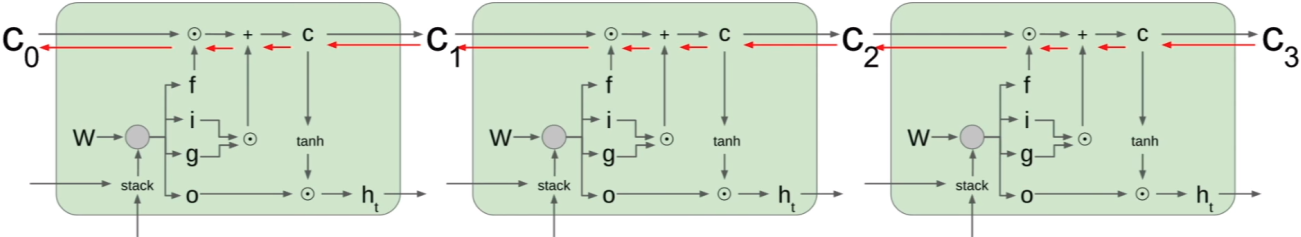
\includegraphics[width=0.99\linewidth]{13_LearningInRecurrentNeuronalNetworks/figures/lstm_many.png}
    \caption{Illustration of LSTM over many sequences. Red arrow denotes the gradient, which can flow uninterruptedly.}
    \label{fig:lstm_many}
\end{figure}

\subsubsection{Gated Recurrent Units (GRUs)}
A Gated Recurrent Unit (GRU) is another way of using gated information in recurrent neural networks. It has fewer parameters than LSTM, as it lacks an output gate. GRU's performance on certain tasks of polyphonic music modeling and speech signal modeling was found to be similar to that of LSTM. GRUs have been shown to exhibit even better performance on certain smaller datasets. An illustration of a GRU is shown below. 

\begin{figure}[H]
    \centering
    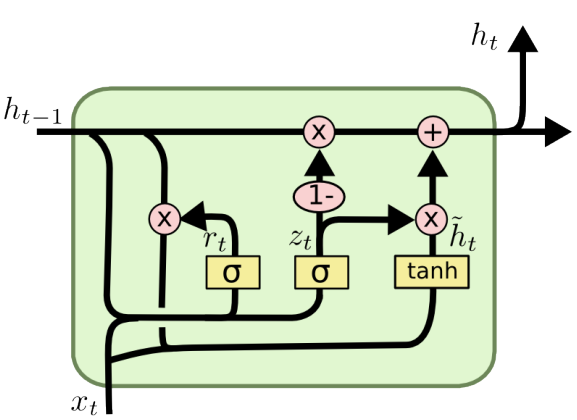
\includegraphics[width=0.6\linewidth]{13_LearningInRecurrentNeuronalNetworks/figures/gru.png}
    \caption{Gated Recurrent Unit (GRU)}
    \label{fig:lstm_many}
\end{figure}

The equations that define the update gate vector $z_t$, the reset gate vector $r_t$ and the output vector $h_t$ are given by

\begin{align*}
&z_{t}=\sigma\left(W_{z} \cdot\left[h_{t-1}, x_{t}\right]\right),\\
&r_{t}=\sigma\left(W_{r} \cdot\left[h_{t-1}, x_{t}\right]\right),\\
&\tilde{h}_{t}=\tanh \left(W \cdot\left[r_{t} * h_{t-1}, x_{t}\right]\right),\\
&h_{t}=\left(1-z_{t}\right) * h_{t-1}+z_{t} * \tilde{h}_{t}.
\end{align*}



\subsection{RNNs in the Brain}
There are claims\footnote{Yamins\&Dicarlo, "Using goal-driven deep learning models to understand sensory cortex", 2016.} that networks of the AlexNet\footnote{Krizhevsky\&Sutskever\&Hinton, "Imagenet classification with deep convolutional neural networks", 2012} type successfully predict properties of neurons in visual cortex. Thus one natural question arises: how similar is an ultra-deep residual network to the primate cortex?\footnote{This paragraph is copied from Liao\&Poggio, "Bridging the Gaps Between Residual Learning, Recurrent Neural Networks and Visual Cortex", 2016} A notable difference is the depth. While a residual network has as many as 1202 layers, biological systems seem to have two orders of magnitude less, if we make the customary assumption that a layer in the NN architecture corresponds to a cortical area. In fact, there are about half a dozen areas in the ventral stream of visual cortex from the retina to the Inferior Temporal cortex. Notice that it takes in the order of 10ms for neural activity to propagate from one area to another one (remember that spiking activity of cortical neurons is usually well below 100 Hz). The evolutionary advantage of having fewer layers is apparent: it supports rapid (100msec from image onset to meaningful information in IT neural population) visual recognition, which is a key ability of human and non-human primates. It is intriguingly possible to account for this discrepancy by taking into account \textbf{recurrent connections within each
visual area}. Areas in visual cortex comprise six different layers with lateral and feedback connections, which are believed to mediate some attentional effects and even learning (such as backpropagation). “Unrolling” in time the recurrent computations carried out by the visual cortex provides an equivalent “ultra-deep”
feedforward network, which might represent a more appropriate comparison with the state-of-the-art computer vision models.
\begin{figure}[H]
    \centering
    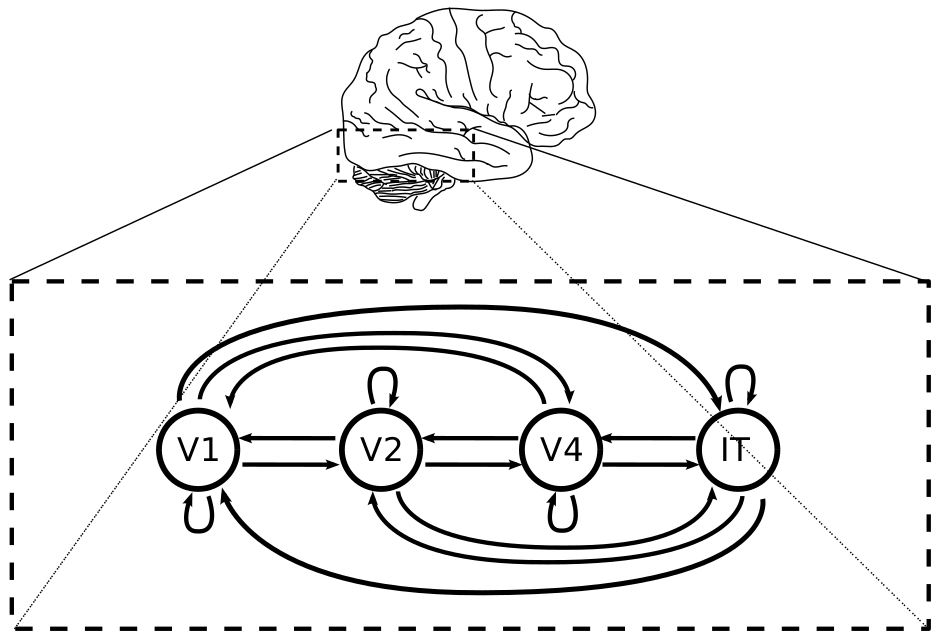
\includegraphics[width=0.7\linewidth]{13_LearningInRecurrentNeuronalNetworks/figures/recurrent_v1to4.png}
    \caption{Multi-state (Fully) Recurrent Neural Network}
    \label{fig:lstm_many}
\end{figure}

\subsubsection{Recurrent Projections in the Cat Brain}
By mapping the circuit of cat primary visual cortex (V1), it is evident, that there are recurrent projections involved\footnote{Binzegger\&Douglas\&Martin, "A Quantitative Map of the Circuit of Cat Primary Visual Cortex", 2004}. 
\subsubsection{Evidence for RNNs in the Rodent Brain}
Similary, it has been shown in rodents, that the communication between columns is organized by multiple highly specific horizontal projection patterns\footnote{Narayanan, "Beyond Columnar Organization: Cell Type- and Target Layer-Specific Principles of Horizontal Axon Projection Patterns in Rat Vibrissal Cortex.", 2015}.

\textbf{Population coding} is a method to represent stimuli by using the joint activities of a number of neurons. In population coding, each neuron has a distribution of responses over some set of inputs, and the responses of many neurons may be combined to determine some value about the inputs.

\hl{...}
\subsubsection{Evidence for RNNs in the Primate Brain}
The brain has both a feed-forward structure and recurrent pathways: Information can get sent back from one area to a previous one or echo around the same area multiple times\footnote{Citing from the webpage that represents the two exercise papers of the lecture: \url{https://www.simonsfoundation.org/2019/05/23/recurrent-connections-improve-neural-network-models-of-vision/}}. Studies suggest this extra processing helps the brain interpret challenging visual information, such as objects that are occluded or viewed from unusual angles. 
A recent study\footnote{Paper from exercise class: Kar\&DiCarlo, "Evidence that recurrent circuits are critical to the ventral stream’s execution of core object recognition behavior", 2019} found images that are difficult for a feed-forward model to classify but easy for humans and monkeys to interpret, although they take slightly longer to classify these challenging images than normal ones. This delay suggests that some recurrent processing is involved. The researchers then looked at how neural activity in the monkey’s brain evolves as these images are processed. A benefit of convolutional neural networks is that the response of different layers in the model can be used to predict the response of neurons in different brain areas. The researchers found that the feed-forward model predicts the activity of neurons fairly well at early stages (up to 0.1 second into the response) but struggles at later time points. When a convolutional neural network is not performing well, researchers in computer vision tend to add more layers to it, making it ‘deeper.’ The authors tested whether such deeper networks could better predict neural responses to their challenging images, under the assumption that a network with more layers, which compute over space, resemble recurrent pathways, which compute over time. These deeper networks were indeed better than the shallower model at predicting neural activity at later time points. Finally, the authors added recurrent connections to the structure of their original model and found that responses at later time points in the model better matched later time points in the data. Specifically, when recurrent connections were added to this ‘shallower’ network, it predicted neural activity as well as the deeper model did. Overall, this work strongly suggests that recurrent processing is an important contributor to computation in the visual system.

\begin{figure}[H]
    \centering
    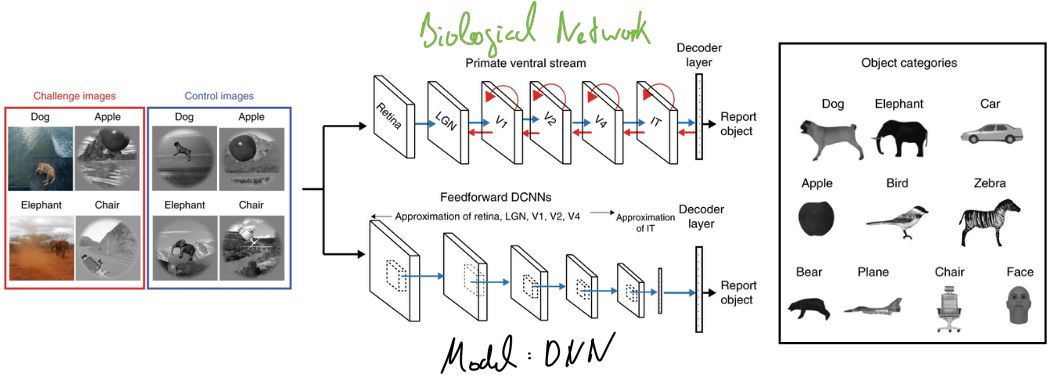
\includegraphics[width=0.99\linewidth]{13_LearningInRecurrentNeuronalNetworks/figures/primate_recognition.png}
    \caption{Both primates (humans and macaques) and feedforward DCNNs were tasked to identify which object is present in each test image (1,320 images). Top: the stages in the primate ventral visual pathway (retina, lateral geniculate nucleus (LGN), areas V1, V2, V4, and the IT cortex), which is implicated in core object recognition. We can conceptualize each stage as rapidly transforming the representation of the image and ultimately yielding the primates’ behavior (that is, producing a behavioral report of which object was present). The blue arrows indicate the known anatomical feedforward projections from one area to the other. The red arrows indicate the known lateral and top-down recurrent connections. Bottom: a schematic of a similar pathway commonly present in DCNNs. These networks contain a series of convolutional and pooling layers with nonlinear transforms at each stage, followed by fully connected layers (which approximate macaque IT neural responses) that ultimately gives rise to the models’ ‘behavior’. Note that the DCNNs only have feedforward (blue) connections.}
    \label{fig:lstm_many}
\end{figure}


\subsection{RNNs in Theoretical Neuroscience}

\subsubsection{Hopfield Network}
A Hopfield network is a form of recurrent artificial neural network popularized by John Hopfield in 1982\footnote{Hopfield, "Neural networks and physical systems with emergent collective computational abilities", 1982}, but described earlier by Little in 1974. Hopfield nets serve as content-addressable (“associative”) memory systems with binary threshold nodes. They are guaranteed to converge to a local minimum, but will sometimes converge to a false pattern (wrong local minimum) rather than the stored pattern (expected local minimum)\footnote{\url{https://pathmind.com/wiki/hopfieldnetworks}}.
%
\begin{figure}[H]
    \centering
    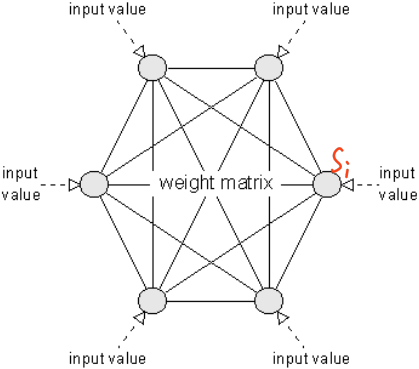
\includegraphics[width=0.6\linewidth]{13_LearningInRecurrentNeuronalNetworks/figures/hopfield.png}
    \caption{Hopfield Network with six units}
    \label{fig:lstm_many}
\end{figure}
%
A Hopfield network has various units, which have a binary state (1/0). The units update asynchronously or synchronously with the following rule:
\[
\begin{array}{ll}
{S_{i}=+1} & {\text { if } \quad x_{i}=\sum_{j \neq i} w_{i j} \cdot S_{j}>\theta_i} \\
{S_{i}=-1} & {\text { if } \quad x_{i}=\sum_{j \neq i} w_{i j} \cdot S_{j}<\theta_i}
\end{array}
\]
Here, $S_i$ is the $i$-th unit of the Hopfield network and $\theta_i$ is the threshold. One can define an energy term as
\begin{equation}
E=-\frac{1}{2} \sum_{i, j} w_{i j} S_{i} S_{j}+\sum_{i} \theta_{i} S_{i}
\end{equation}
With each update step, the energy either stays constant or decreases. 

\subsubsection{Reservoir Computing}
Reservoir computing is a framework for computation that may be viewed as an extension of neural networks. Typically an input signal is fed into a fixed (random) dynamical system called a reservoir (for example a RNN). Hereby, the dynamics of the reservoir map the input to a higher dimension. Then a simple readout mechanism is trained to read the state of the reservoir and map it to the desired output. The main benefit is that training is performed only at the readout stage and the reservoir is fixed\footnote{\url{https://en.wikipedia.org/wiki/Reservoir_computing}}. A really cool thought is, that basically every (abstract or physical) dynamic system can be used as the reservoir\footnote{Tanaka, "Recent Advances in Physical Reservoir Computing:
A Review", 2019}, including a water tank\footnote{Fernando\&Sojakka, "Pattern Recognition in a Bucket", 2003}, an electronic circuit or parts of the brain itself! 

\paragraph{Echo State Network:} Recurrent neural network with a random and sparsely connected (~1\%) hidden layer / reservoir, works in discrete time, different activity update modes.

\paragraph{Liquid State Machine:} Biologically plausible, spiking RNN reservoir, randomly connected, continuous in time, asynchronous integration, uses linear discriminate units.

\begin{figure}[H]
    \centering
    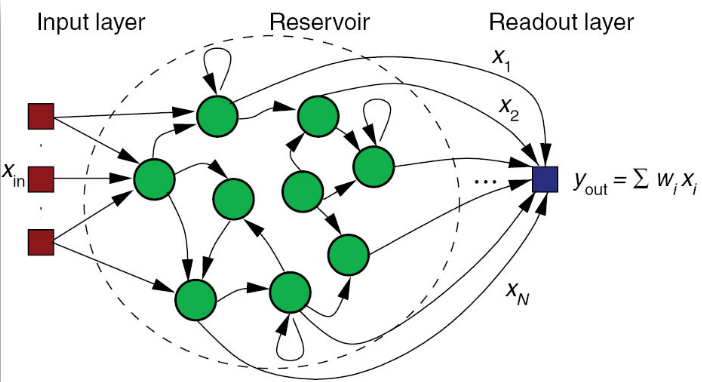
\includegraphics[width=0.8\linewidth]{13_LearningInRecurrentNeuronalNetworks/figures/reservoir.png}
    \caption{Reservoir computing}
    \label{fig:lstm_many}
\end{figure}

\subsubsection{Learning Algorithms}
\paragraph{Learning via Backpropagation Through Time (BPTT):}

See above.
\hl{...}

\paragraph{Learning via Real Time Recurrent Learning (RTRL):}
A general approach to training an arbitrary recurrent network by adjusting weights along the error gradient. This algorithm usually requires very low learning rates because of the inherent correlations between successive node outputs.

\hl{...}

\paragraph{First-Order, Reduced and Controlled Error (FORCE) Learning:}

\hl{...}

\begin{figure}[H]
    \centering
    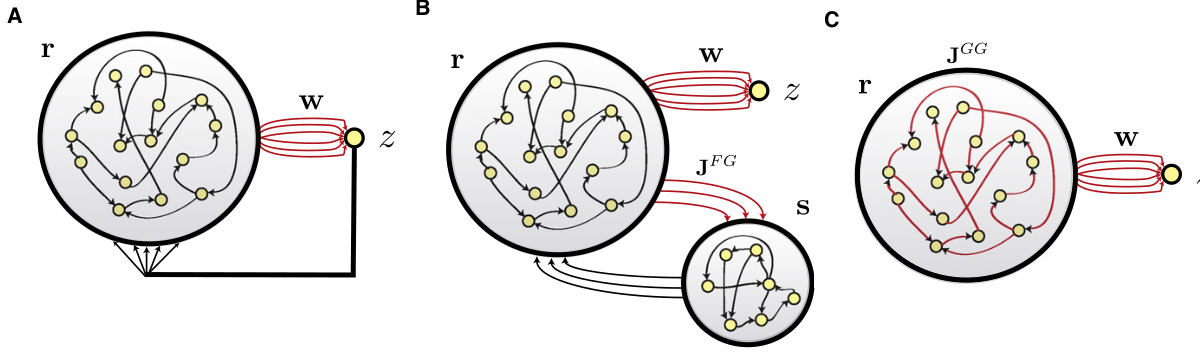
\includegraphics[width=0.99\linewidth]{13_LearningInRecurrentNeuronalNetworks/figures/force.png}
    \caption{First-Order, Reduced and Controlled Error (FORCE) Learning. In all three cases, a recurrent generator network with firing rates \textbf{r} drives a linear
    readout unit with output $z$ through weights \textbf{w} (red) that are modified during training. Only connections shown in red are subject to modification. \textbf{(A)} Feedback to the generator network (large network circle) is provided by the readout unit. \textbf{(B)} Feedback to the generator network is provided by a separate feedback network (smaller network circle). Neurons of the feedback network are recurrently connected and receive input from the generator network through synapses of strength $J^{FG}$ (red), which are modified during training. \textbf{(C)} A network with no external feedback. Instead, feedback is generated within the network and modified by applying FORCE learning to the synapses with strengths $J^{GG}$ internal to the network (red).}
    \label{fig:force}
\end{figure}


\paragraph{Self Organizing Recurrent Networks (SORN)}
It combines three distinct forms of local plasticity to learn spatio-temporal patterns in its input while maintaining its dynamics in a healthy regime suitable for learning\footnote{Lazar, "A Self-Organizing Recurrent Neural Network", 2009}. The SORN learns to encode information in the form of trajectories through its high-dimensional state space reminiscent of recent biological findings on cortical coding. All three forms of plasticity are shown to be essential for the network's success:
\begin{enumerate}
    \item STDP Rule
    \item Weight Normalization Rule
    \item Distributed Processing Rule
\end{enumerate}

\begin{figure}[H]
    \centering
    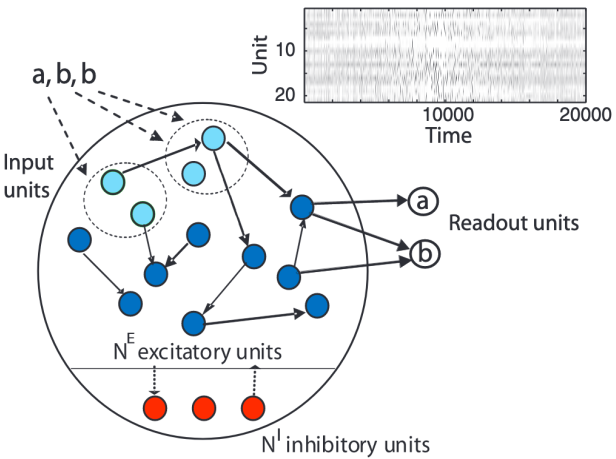
\includegraphics[width=0.6\linewidth]{13_LearningInRecurrentNeuronalNetworks/figures/sorn.png}
    \caption{Self Organizing Recurrent Networks (SORN)}
    \label{fig:sorn}
\end{figure}

\end{document}